\subsection{Общее описание мониторинга}\label{subsec:-monitoringall-}
Мониторинг организован с помощью:

\begin{itemize}
    \item \textbf{postgres\_exporter} - инструмента, который выполняет запросы к базе, подключаясь под
    специально созданным юзером с ограниченными правами.
    \item \textbf{Prometheus} - известного сборщика метрик, обращающегося по http к postgres\_exporter.
    \item \textbf{Grafana} - инструмента визуализации метрик.
\end{itemize}

В качестве изюминки проекта было реализовано предварительное встраивание панелей (дашбордов)
при разворачивании образа grafana, делая проект готовым к демонстрации уже ``с порога``.
Готовая красивая панель для postgresql была скачана с сайта grafana.

\begin{figure}[htbp]
    \centering
    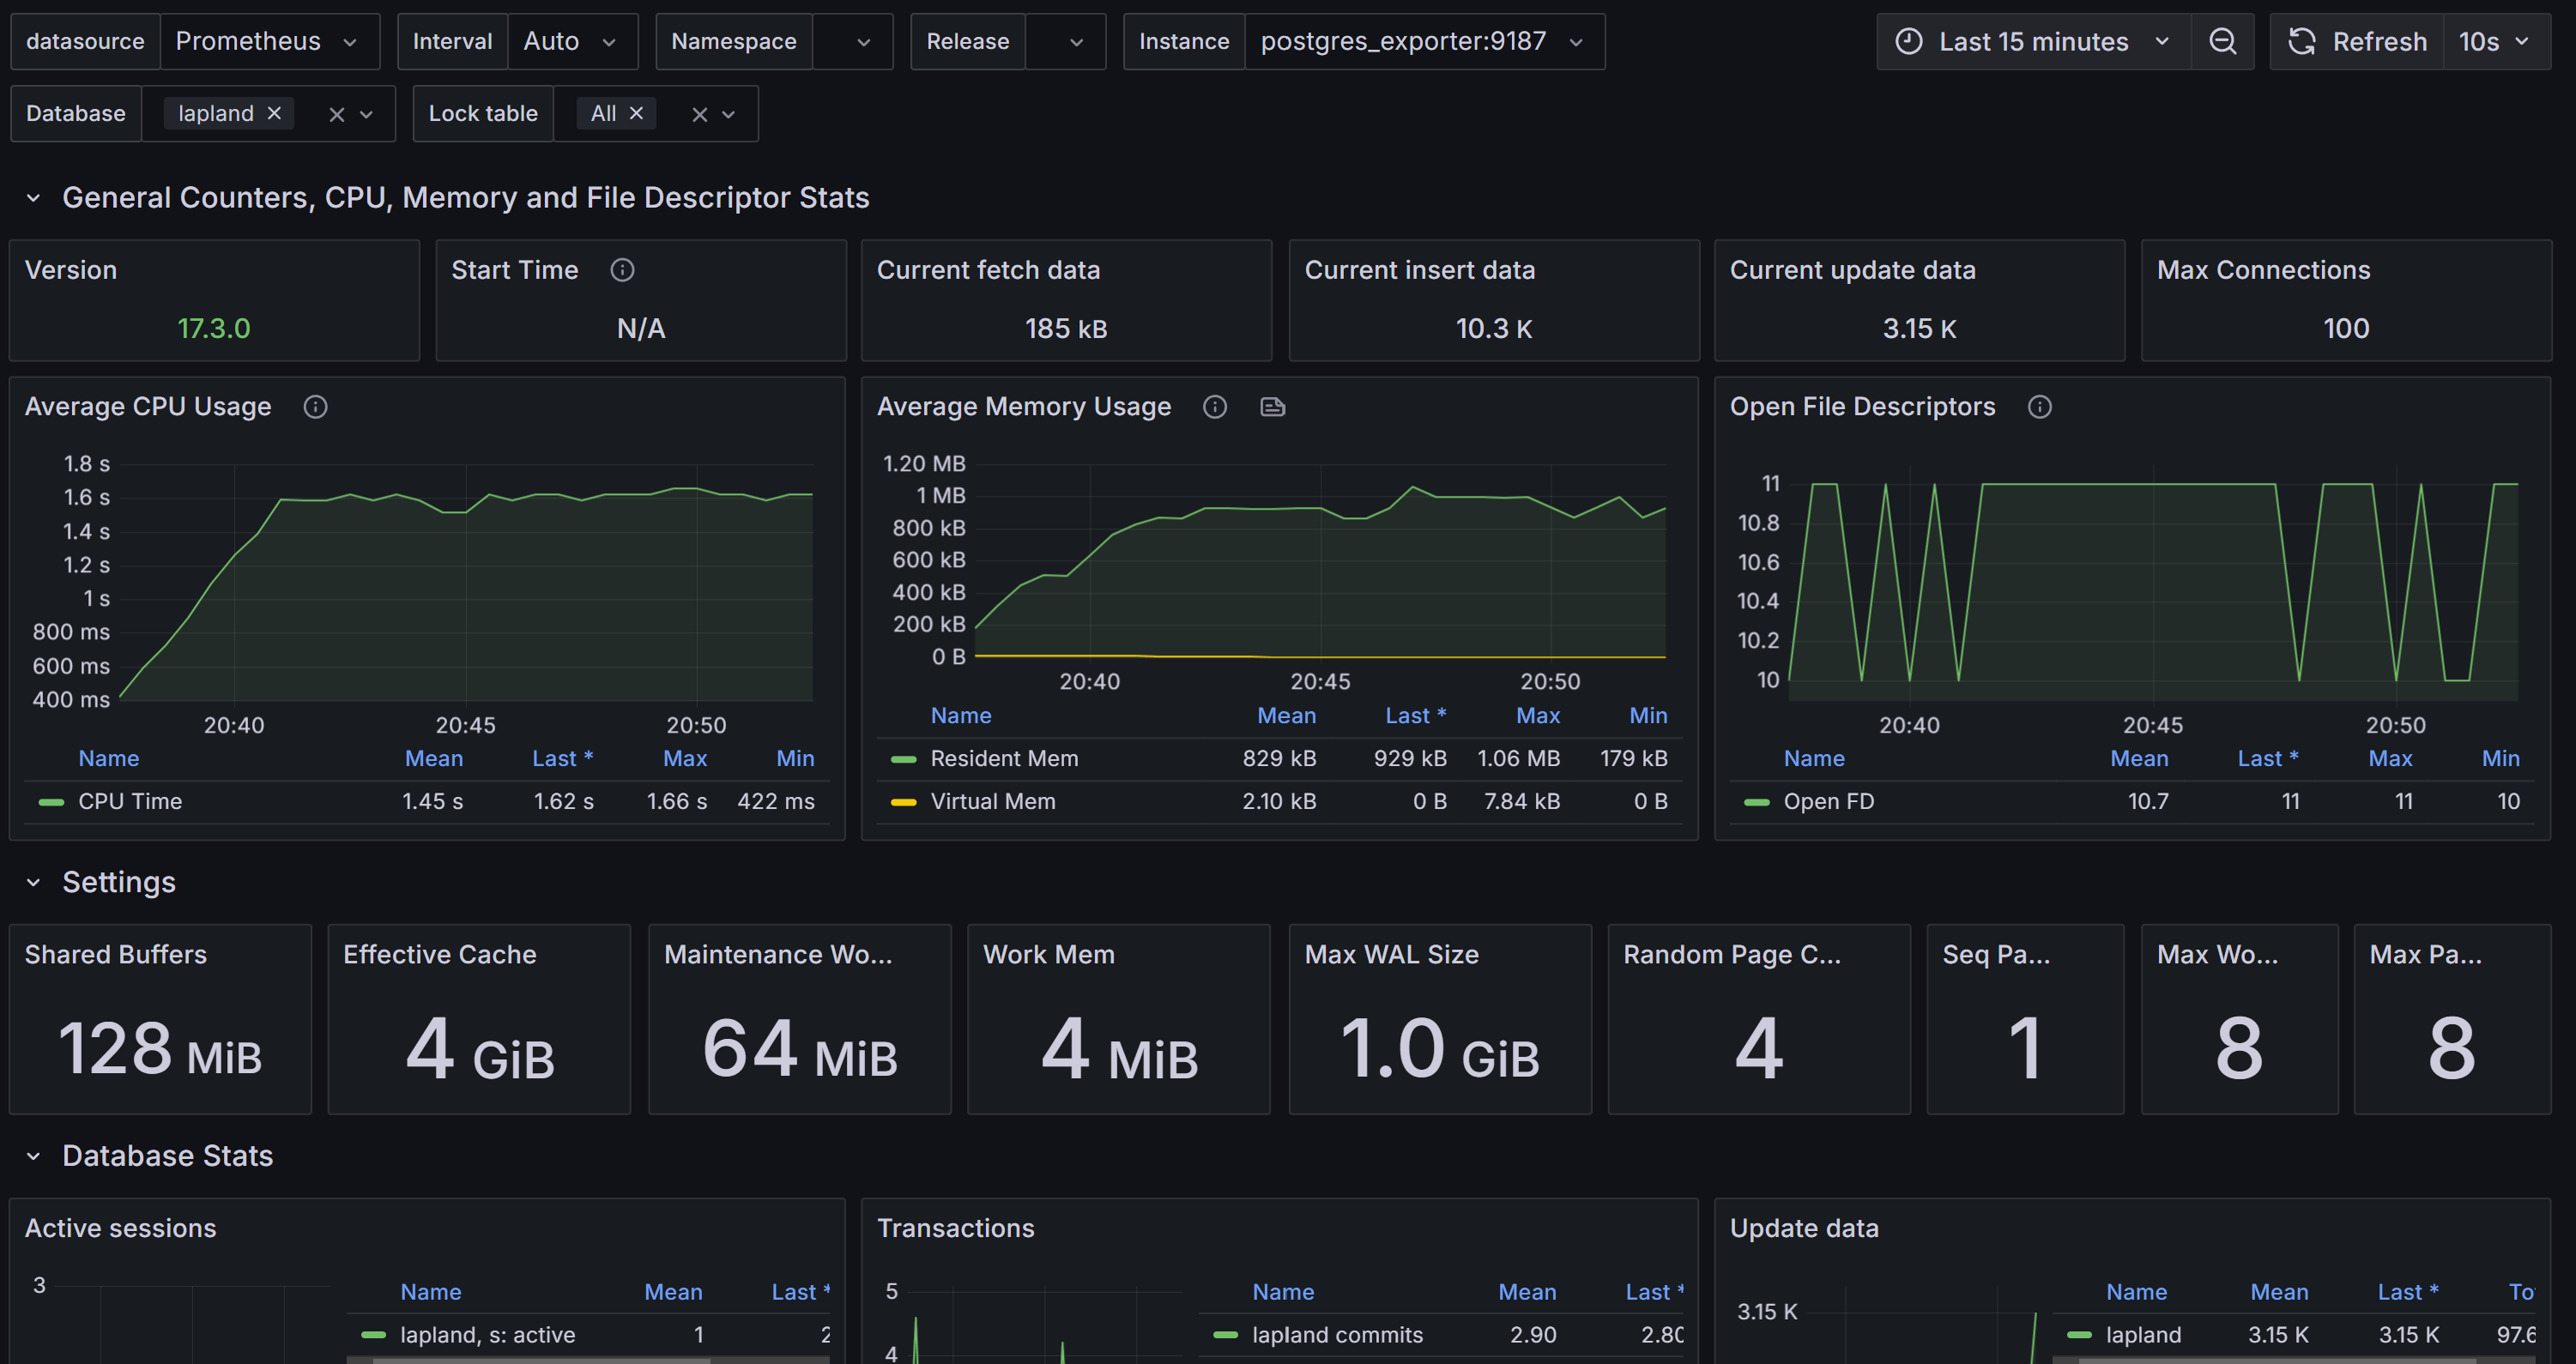
\includegraphics[width=0.9\textwidth]{grafana} % Вставка изображения
    \caption{Панель мониторинга в Grafana}\label{fig:grafanapic}
\end{figure}